\section{目的}
本研究では, 地理的分散環境下における RW 実行エンジンを提案した. 提案手法を既存の分散 RW 実行エンジンである KnightKing \cite{10.1145/3341301.3359634} と比較することで, 地理的分散環境下における本手法の有用性を明らかにする. また, 実行する RW の終了確率を変えたときの評価や, 送信時に RWer をまとめない場合との比較, そして経路再利用のための再利用エッジデータが貯まるまでの RW 実行数の評価を行うことで, 本手法の構成要素に関する性能調査も行った. 

\section{項目}

評価項目は以下の通りである. 
\begin{quote}
    \begin{itemize}
     \item RTT, パケットロス率を変えた場合の実行時間
     \item Random Walker の経路再利用をした場合の実行時間
     \item グラフ分割の汚さを変えた場合の実行時間
     \item グラフ分割数を変えた場合の実行時間
     \item 終了確率 $\alpha$ を変えた場合の実行時間
     \item Random Walker をまとめて送信した場合とそうでない場合の実行時間
     \item 再利用エッジが貯まるまでに実行する Random Walk 実行数
    \end{itemize}
\end{quote}

\section{評価環境}

\subsection{データセット}

本評価では実世界グラフと生成グラフの両方を使用して実験を行った. 実世界グラフは LiveJournal のデータセット\cite{snapnets} (頂点数 3,997,962, 辺数 69,362,378) を使用した. 生成グラフに関しては, エッジ生成確率を制御できるアルゴリズムである, Stochastic block model (SBM) \cite{SBM} を使用した. SBM では, partition 数, 各 partition 内の頂点数, partition 内の頂点間のエッジ生成確率, partition 間の頂点間のエッジ生成確率を指定し, グラフを生成することができる. このエッジ生成確率を操作することで, 例えばサーバ間を跨ぐ RW 遷移が多くなるグラフを生成することができる. 生成グラフの頂点数とエッジ生成確率の値に関しては, 実験 \ref{グラフ分割の汚さを変えた場合の実行時間}, \ref{グラフ分割数を変えた場合の実行時間} で説明する. 

\subsection{評価環境}

本評価では最大 7 台のサーバを使用して実験を行った. 各サーバは全て同じ性能をしており, 表 \ref{評価環境} に示す. また, 実装は全て C++ で行った. 

\begin{table}[t]
    \caption{評価環境}
    \label{評価環境}
    \centering
    \begin{tabular}{c|c}
      \hline
      項目 & 内容   \\
      \hline \hline
      OS  & Ubuntu 20.04 LTS \\
      CPU  & Intel(R) Xeon(R) CPU E5-2643 v2 @ 3.50GHz  \\
      Core & 24 (hyper threading 有効) \\
      RAM  & 32GB \\
      \hline
    \end{tabular}
\end{table}

\subsection{RW 実行について}

本評価における RW 実行のに実行時間について, 開始時間は RWer を生成し始めるタイミングで, 終了時間は全てのサーバで全ての RWer の終了確認が取れたタイミングとしている. 既存手法と異なり提案手法は UDP 通信を使用しているため, パケットロスによる RWer の損失が発生する. 本来提案手法では, RWer の損失の影響が少ない (図 \ref{局所的に RWer が損失したときの PPR 演算の精度} 参照) ことを理由にパケットロスを許容しているが, 全ての RWer の終了を前提としている既存手法との比較のために, 簡易的な再送機能を実装した. 再送スレッドは全体の 95 \% の RW 実行が終了した時点で起動し, 3 秒ごとにまだ終了確認の取れてない RWer を再生成する.  

\section{RTT, パケットロス率を変えた場合の実行時間}\label{RTT, パケットロス率を変えた場合の実行時間}

データセットは実世界グラフ, サーバ数は 5 台で実験を行った. まず, 実験前にグラフを 5 分割し, 各サーバに配置する. ここでの分割方法はハッシュ分割 (ランダム分割) である. 具体的には, 各サーバの ID を 0 $\sim$ 4 とし, 各頂点をサーバ ID = 頂点 ID \% 5 のサーバに配置する. この先特に指定がない場合は, 分割に関してはこのハッシュ分割を採用している. そして RW 実行に関しては, 終了確率 $\alpha$ の RW を各頂点から 10 回ずつ実行する. 実世界グラフの頂点数は 3,997,962 なので実行する RW 数は合計 39,979,620 回となる. 実験結果を図 \ref{パケットロス率を 0.03 に固定したときの実行時間}, \ref{RTT を 100 ms に固定したときの実行時間} に示す. まず, 図 \ref{パケットロス率を 0.03 に固定したときの実行時間} は, サーバ間のパケットロス率を 0.03 \% に固定し, RTT を 0 $\sim$ 200 ms で変動させて実験を行った結果である. 既存手法では RTT が 0 ms, 50 ms, 100 ms, 150 ms, 200 ms と変化すると実行時間が約 4 秒, 52 秒, 86 秒, 131 秒, 151 秒となり, 大幅に増加していることがわかる. これは既存手法が TCP 通信を使用していることが原因であり, RTT が大きくなるとスループットが小さくなる. 対して提案手法では RTT が 0 ms, 50 ms, 100 ms, 150 ms, 200 ms と変化すると実行時間が約 49 秒, 52 秒, 53 秒, 55 秒, 55 秒となっており, 既存手法と比べてあまり増加しないことがわかる. これは提案手法が UDP 通信を使用しているためであり, RTT が変化してもスループットの変化は小さい. RTT が 0 のときは既存手法が 4 秒, 提案手法が 49 秒と既存手法の方が約 12 倍高速である. これは, 既存手法における RWer の送信では経路情報を送らないため通信量が少ないこと, そして同期処理によって CPU リソースを最大限活用することができていることが要因であると考える. 図 \ref{RTT を 100 ms に固定したときの実行時間} は, サーバ間の RTT を 100 ms に固定し, パケットロス率を 0 $\sim$ 0.1 \% で変動させて実験を行った結果である. こちらも 図 \ref{パケットロス率を 0.03 に固定したときの実行時間} と同様に, パケットロス率の増加とともに実行時間が大きく増加する既存手法に対し, 提案手法では実行時間がほとんど変化していない. これらの結果から, RTT, パケットロス率が無視できるような環境では既存手法のような TCP 通信を使った同期処理による RW 処理, 地理的分散環境のような RTT, パケットロス率が無視できない環境では提案手法のような UDP 通信を使った非同期処理が適していることがわかる. 

\begin{figure}[t]
    \centering
    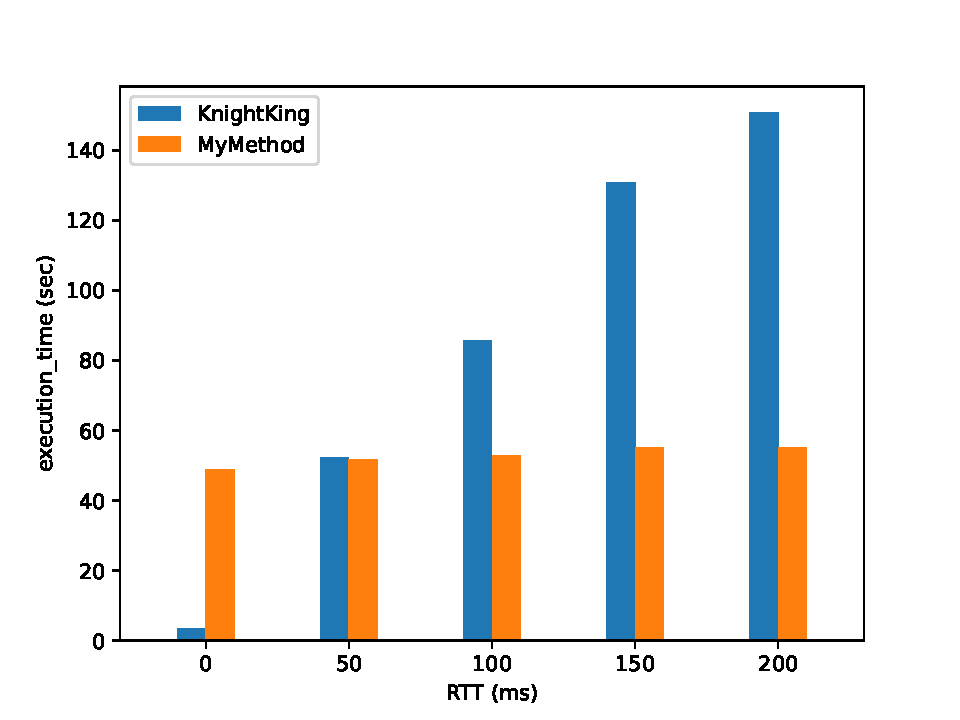
\includegraphics[scale=0.8]{figure/Kn_vs_AR_RTT.pdf}
    \caption{パケットロス率を 0.03 \% に固定したときの実行時間}
    \label{パケットロス率を 0.03 に固定したときの実行時間}
\end{figure}

\begin{figure}[t!]
    \centering
    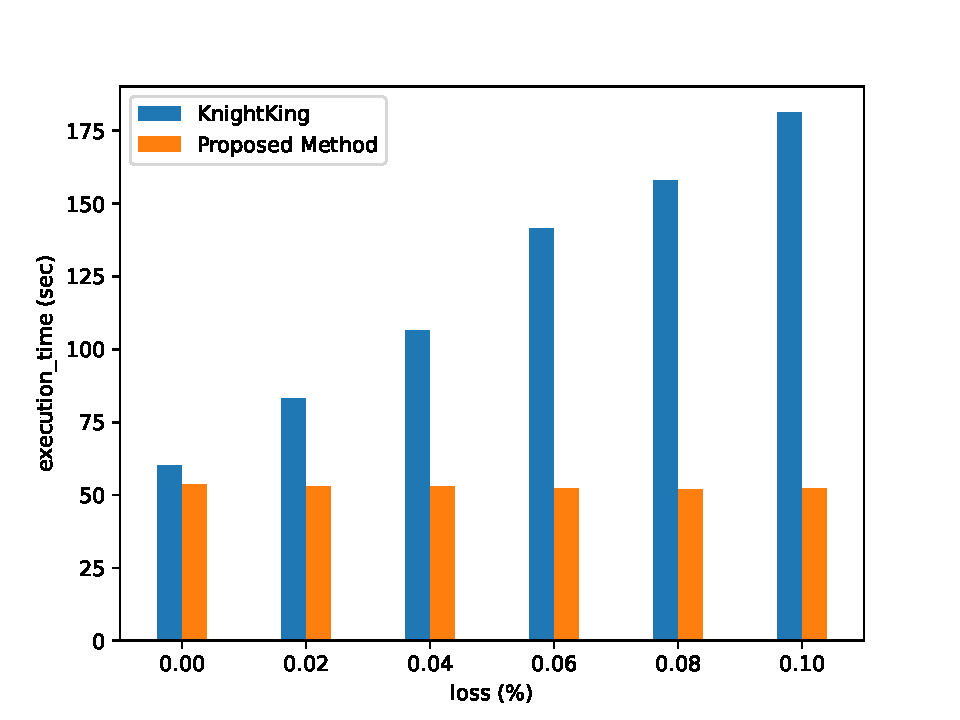
\includegraphics[scale=0.8]{figure/Kn_vs_AR_loss.pdf}
    \caption{RTT を 100 ms に固定したときの実行時間}
    \label{RTT を 100 ms に固定したときの実行時間}
\end{figure}

\section{Random Walker の経路再利用をした場合の実行時間}\label{Random Walker の経路再利用をした場合の実行時間}

データセットは実世界グラフ, サーバ数は 5 台で実験を行った. RW 実行に関しては \ref{RTT, パケットロス率を変えた場合の実行時間} と同様で, 終了確率 $\alpha$ の RW を各頂点から 10 回ずつ実行する. また, RTT は 100 ms, パケットロス率は 0.03 \% でそれぞれ固定し, 再利用するためのエッジデータは実験前に調達済みであるとする. 図 \ref{経路再利用をしたときの実行時間} に経路再利用をしたときの実験結果を示す. 緑の点線は既存手法を, 青い棒は提案手法の経路再利用をしないもの, オレンジ色の棒は提案手法の経路再利用をするものを表す. 横軸における original edges は元々各サーバが保持していたエッジの数であり, reuse edges は再利用エッジの数である. 実世界グラフにおけるエッジの数は全部で 69,362,378 なので, これを 5 分割した約 14,000,000 が original edges の値となる. つまり, original edges + reuse edges = 20,000,000 のとき, reuse edges の値は約 6,000,000 である. 実験結果について, 提案手法の経路再利用をしない場合は既存手法に比べて約 1.6 倍高速であり, 提案手法の経路再利用をする場合はそれぞれ提案手法に比べて約 2.2 倍, 2.9 倍, 3.8 倍, 5.0 倍, 7.2 倍高速だった. 結果から RWer の経路再利用により実行時間を削減できていることがわかる. また, 経路再利用による削減時間を再利用エッジ数で割ることにより, 再利用エッジ 1 本あたりの時間削減量を求めたところ, original edges + reuse edges ($\times$ 10000) = 2000, 3000, 4000, 5000, 6000 でそれぞれ約 0.024, 0.014, 0.012, 0.010, 0.009 になった. この結果から, 再利用エッジが増えれば増えるほど再利用エッジ 1 本あたりの時間削減量が減ることがわかった. 

\begin{figure}[t]
    \centering
    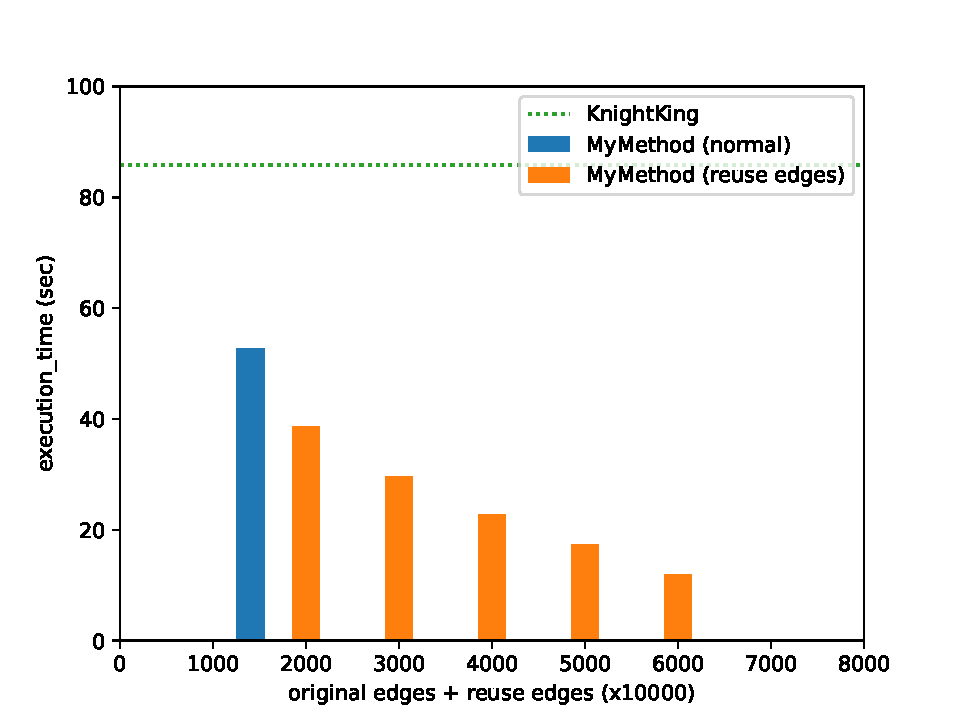
\includegraphics[scale=0.8]{figure/AR_cache.pdf}
    \caption{経路再利用をしたときの実行時間}
    \label{経路再利用をしたときの実行時間}
\end{figure}

\section{グラフ分割の汚さを変えた場合の実行時間}\label{グラフ分割の汚さを変えた場合の実行時間}

a

\section{グラフ分割数を変えた場合の実行時間}\label{グラフ分割数を変えた場合の実行時間}

\section{終了確率 $\alpha$ を変えた場合の実行時間}\label{終了確率 alpha を変えた場合の実行時間}

\section{Random Walker をまとめて送信した場合とそうでない場合の実行時間}\label{Random Walker をまとめて送信した場合とそうでない場合の実行時間}

\section{再利用エッジが貯まるまでに実行する Random Walk 実行数}\label{再利用エッジが貯まるまでに実行する Random Walk 実行数}